\begin{exr}{}
La reacció que té lloc en una bateria d'ió liti com la de la imatge
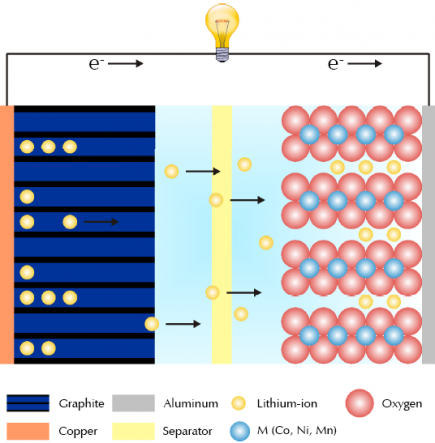
\includegraphics[scale=0.5]{LiIon.png}
és \ch{LiC6 + CoO2 <=> LiCoO2 + C6}. Escriu les dues mitges reaccions i fes-hi el balanç. Calcula el potencial de cel·la a partir de la $\Delta \varepsilon^{\circ}$ del \ch{Li+} (-3.0V) i del \ch{CoO2} (+1.1V).
Quins valors obtindries per a la reacció que tindria lloc en una bateria de Li i \ch{O2} ($\Delta \varepsilon^{\circ}$ de la reacció \ch{O2_{(g)} + 2 H+ + 2 e- -> H2O2_{(aq)}} és 0.3V).
\end{exr}
